\documentclass{article}
\usepackage[T1]{fontenc}
\usepackage{lmodern}
\usepackage{graphicx}
\usepackage{amsmath,amssymb}
\usepackage[a4paper,margin=2cm]{geometry}
\usepackage[absolute,overlay]{textpos}
\setlength{\TPHorizModule}{1mm}
\setlength{\TPVertModule}{1mm}
\usepackage[indonesian]{babel}
\usepackage{hyperref}
\setlength{\emergencystretch}{2em}
% unit: Halaman 47

\begin{document}

% === Halaman 47 (llm) ===

% (tidak ada teks dari model)

% deskripsi: Diagram ilustrasi algoritma RC4 yang menunjukkan proses pemutakhiran S-box, termasuk operasi swap antara elemen S[i] dan S[j], serta penghitungan indeks t menggunakan rumus (S[i] + S[j]) mod 256.
% bbox normalisasi: [0.1500, 0.2500, 0.8500, 0.6000]
\begin{textblock*}{147.00mm}(31.50mm,74.25mm)
\noindent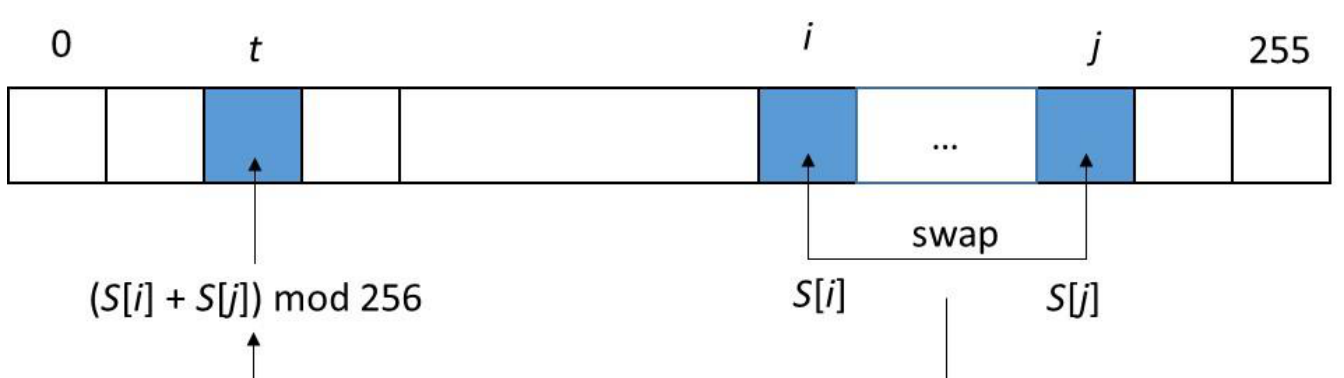
\includegraphics[width=147.00mm,height=103.95mm]{../../images/llm/page_047_img_01.png}%
\end{textblock*}

\end{document}
